\documentclass[12pt,a4paper]{article}

% ── Packages ──────────────────────────────────────────────────────────────────
\usepackage[T1]{fontenc}
\usepackage[utf8]{inputenc}
\usepackage{lmodern}
\usepackage[margin=2.5cm]{geometry}
\usepackage{amsmath,amssymb}
\usepackage{booktabs}
\usepackage{array}
\usepackage{multirow}
\usepackage{xcolor}
\usepackage{hyperref}
\usepackage{graphicx}
\usepackage{float}
\usepackage{caption}
\usepackage{subcaption}
\usepackage{enumitem}
\usepackage{titlesec}
\usepackage{parskip}
\usepackage{microtype}
\usepackage{pgfplots}
\usepackage{pgfplotstable}
\usepackage{tikz}
\pgfplotsset{compat=1.18}

% ── Colours ───────────────────────────────────────────────────────────────────
\definecolor{mitblue}{RGB}{0,51,102}
\definecolor{lightgray}{RGB}{245,245,245}
\definecolor{darkgray}{RGB}{80,80,80}
\definecolor{rfgreen}{RGB}{34,139,34}
\definecolor{knnblue}{RGB}{30,100,200}
\definecolor{sgdorange}{RGB}{210,100,10}
\definecolor{svcred}{RGB}{180,30,30}

% ── Section formatting ────────────────────────────────────────────────────────
\titleformat{\section}{\large\bfseries\color{mitblue}}{{\thesection.}}{0.5em}{}[\vspace{-4pt}\rule{\linewidth}{0.8pt}]
\titleformat{\subsection}{\normalsize\bfseries\color{mitblue}}{\thesubsection}{0.5em}{}
\titleformat{\subsubsection}{\normalsize\bfseries\color{darkgray}}{\thesubsubsection}{0.5em}{}

% ── Hyperref setup ────────────────────────────────────────────────────────────
\hypersetup{
  colorlinks=true,
  linkcolor=mitblue,
  citecolor=mitblue,
  urlcolor=mitblue,
  pdftitle={Late Delivery Risk Classification -- CS280 Lab Report},
  pdfauthor={Supply Chain Team}
}

% ══════════════════════════════════════════════════════════════════════════════
\begin{document}

% ── Title page ────────────────────────────────────────────────────────────────
\begin{titlepage}
  \centering
  \vspace*{1.5cm}
  {\Large\bfseries Mediterranean Institute of Technology\\[4pt]
   \large CS280 --- Introduction to Artificial Intelligence\\[2pt]
   \normalsize Spring 2026}\\[2cm]

  \rule{\linewidth}{1.5pt}\\[0.4cm]
  {\LARGE\bfseries\color{mitblue}
    Late Delivery Risk Classification\\[6pt]
    in Supply Chain Logistics}\\[0.4cm]
  \rule{\linewidth}{1.5pt}\\[1.5cm]

  {\large\bfseries Lab Project Report}\\[0.5cm]
  {\normalsize DataCo Global Supply Chain Dataset}\\[2cm]

  \begin{tabular}{ll}
    \textbf{Domain}     & Business / Supply Chain \\[4pt]
    \textbf{Course}     & CS280 \\[4pt]
    \textbf{Instructor} & Mohamed Iheb Hergli \\[4pt]
    \textbf{Semester}   & Spring 2026 \\[4pt]
    \textbf{Date}       & April 2026 \\
  \end{tabular}

  \vspace{1.5cm}
  {\normalsize\bfseries Team Members}\\[0.5cm]
  \begin{tabular}{c}
    Imen Boukadida \\[3pt]
    Lina Khemiri \\[3pt]
    Cyrine Krichen \\[3pt]
    Mohamed Garouachi \\[3pt]
    Youssef Ben Jemaa \\
  \end{tabular}

  \vfill
  {\normalsize Mediterranean Institute of Technology}
\end{titlepage}

% ── Table of Contents ─────────────────────────────────────────────────────────
\tableofcontents
\newpage

% ══════════════════════════════════════════════════════════════════════════════
\section{Introduction}
\label{sec:intro}

Late deliveries are a persistent and costly challenge in global supply chain
management. Missed shipping deadlines reduce customer satisfaction, erode
margins, and trigger contractual penalties. The ability to \emph{predict}
whether an order will arrive late---before it is shipped---gives logistics
teams the opportunity to intervene proactively: re-routing shipments,
pre-allocating express capacity, or issuing early customer notifications.

This project addresses late delivery prediction as a \textbf{binary
classification problem}. Given a set of order-level features available at the
time of dispatch (shipping mode, product category, geographic coordinates,
financial metrics, and temporal attributes), the objective is to predict
whether the order will be delivered on time ($y=0$) or late ($y=1$).

The project follows a complete machine learning pipeline:
\begin{enumerate}[leftmargin=2em,itemsep=2pt]
  \item Exploratory data analysis and preprocessing
  \item Stratified train/test split with inference holdout
  \item Training and hyperparameter tuning of four distinct models
  \item Scientific evaluation and benchmarking
  \item Final model selection with justification
  \item Inference on 10 unseen production orders
\end{enumerate}

All work was conducted in Python using scikit-learn, pandas, and matplotlib,
inside a Jupyter notebook as required by the course guidelines.

% ══════════════════════════════════════════════════════════════════════════════
\section{Background}
\label{sec:background}

\subsection{Dataset}

The \textbf{DataCo Global Supply Chain Dataset} is a publicly available
real-world dataset containing transactional records from a global distributor.
After removing the 10 held-out inference rows (extracted before any
preprocessing), the working dataset comprises \textbf{180,509 orders} with
features spanning shipping logistics, product information, geographic
coordinates, and financial metrics.

\paragraph{Target variable.}
\texttt{Late\_delivery\_risk} is a binary indicator:
\begin{itemize}[itemsep=2pt]
  \item \textbf{Class 0 --- On-Time:} 81,481 records (45.2\,\%)
  \item \textbf{Class 1 --- Late:} 99,028 records (54.8\,\%)
\end{itemize}

The moderate class imbalance (54.8\,\% positive) is not severe enough to
require resampling, but it motivates the choice of \textbf{F1-score} as the
primary evaluation metric rather than raw accuracy.

Figure~\ref{fig:class_dist} shows the class distribution.

\begin{figure}[H]
\centering
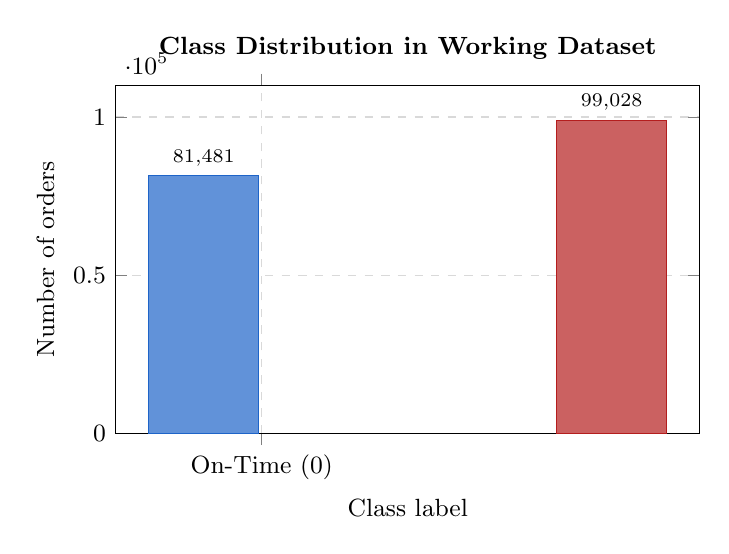
\begin{tikzpicture}
\begin{axis}[
  ybar,
  bar width=1.4cm,
  width=9cm, height=6cm,
  symbolic x coords={On-Time (0), Late (1)},
  xtick=data,
  ymin=0, ymax=110000,
  ylabel={Number of orders},
  ylabel style={font=\small},
  xlabel={Class label},
  xlabel style={font=\small},
  tick label style={font=\small},
  nodes near coords,
  nodes near coords align={vertical},
  every node near coord/.append style={font=\scriptsize},
  enlarge x limits=0.5,
  grid=major,
  grid style={dashed,gray!30},
  title={Class Distribution in Working Dataset},
  title style={font=\small\bfseries},
]
\addplot[fill=knnblue!70, draw=knnblue] coordinates {(On-Time (0), 81481)};
\addplot[fill=svcred!70,  draw=svcred]  coordinates {(Late (1),     99028)};
\end{axis}
\end{tikzpicture}
\caption{Class distribution of \texttt{Late\_delivery\_risk} after holdout extraction.}
\label{fig:class_dist}
\end{figure}

\subsection{Related Work and Learning Paradigm}

Delivery risk prediction is a well-studied problem in supply chain analytics.
Prior work typically frames it as a supervised binary classification task,
using models ranging from logistic regression and decision trees to gradient
boosting ensembles. This project deliberately spans a range of algorithmic
families---distance-based, linear, and ensemble---to enable meaningful
scientific comparison, as required by the course guidelines.

% ══════════════════════════════════════════════════════════════════════════════
\section{Methodology}
\label{sec:methodology}

\subsection{Preprocessing Pipeline}

The preprocessing pipeline was designed to prevent data leakage and to mirror
production conditions. All fitting (encoding, scaling, imputation statistics)
was performed exclusively on the training set and then applied to the test set
and inference holdout.

\begin{enumerate}[leftmargin=2em,itemsep=3pt]
  \item \textbf{Inference holdout extraction.} Ten rows were randomly sampled
        \emph{before} any preprocessing and stored as the inference set,
        simulating production data arriving with no prior processing.
  \item \textbf{Leakage column removal.} Features only available
        post-shipment (e.g., actual delivery date) were dropped.
  \item \textbf{Temporal feature engineering.} Order dates were parsed and
        decomposed into \texttt{order\_month}, \texttt{order\_dayofweek},
        and \texttt{order\_quarter}.
  \item \textbf{Missing value imputation.} Forward-fill followed by linear
        interpolation; imputation state persisted for the inference set.
  \item \textbf{Outlier handling.} Winsorization at the 1st and 99th
        percentiles on all numerical features.
  \item \textbf{Near-zero variance removal.} Constant or quasi-constant
        columns dropped.
  \item \textbf{Correlation-based filtering.} Highly correlated numerical
        feature pairs removed (redundant features discarded).
  \item \textbf{Rare category grouping.} Infrequent categorical levels
        collapsed into an \texttt{Other} bucket.
  \item \textbf{Train--test split.} 80\,\% training / 20\,\% test,
        stratified on the target, \texttt{random\_state=42}.
  \item \textbf{One-hot encoding.} \texttt{OneHotEncoder(handle\_unknown=
        'ignore')} fitted on training set; applied to all splits.
  \item \textbf{Numerical scaling.} \texttt{RobustScaler} fitted on training
        set; applied to all splits.
\end{enumerate}

After preprocessing, the final feature matrix has \textbf{232 features}:

\begin{table}[H]
\centering
\caption{Dataset dimensions after preprocessing.}
\label{tab:dataset_dims}
\begin{tabular}{lrr}
\toprule
\textbf{Split} & \textbf{Rows} & \textbf{Features} \\
\midrule
Training set   & 144,407 & 232 \\
Test set       &  36,102 & 232 \\
Inference holdout &    10 & 232 \\
\bottomrule
\end{tabular}
\end{table}

\subsection{Models}

Four models with genuinely distinct algorithmic principles were implemented,
fulfilling the mandatory requirement of at least three distinct architectures.

\subsubsection{k-Nearest Neighbours (k-NN)}

k-NN is a non-parametric, instance-based algorithm. For a query point
$\mathbf{x}$, prediction is determined by majority vote among the $k$ closest
training examples under a chosen distance metric:
\[
  \hat{y} = \underset{c}{\operatorname{arg\,max}}
            \sum_{i \in \mathcal{N}_k(\mathbf{x})} w_i \,\mathbf{1}[y_i = c]
\]
where $w_i$ is a distance-based weight when \texttt{weights='distance'}.
Because k-NN stores all training points, it was trained on a stratified
subsample of 25,000 rows to keep inference tractable on 232 features.

\subsubsection{Stochastic Gradient Descent Classifier (SGD)}

The SGDClassifier with \texttt{loss='modified\_huber'} learns a linear
decision boundary by minimising the regularised empirical risk online:
\[
  \min_{\mathbf{w}} \; \frac{1}{n}\sum_{i=1}^{n} \ell_{\text{mH}}
  (y_i, \mathbf{w}^\top \mathbf{x}_i) + \alpha \|\mathbf{w}\|_2^2
\]
The Modified Huber loss is smooth at the margin boundary and naturally
supports probability estimates, making it suitable for a probabilistic
comparison with other models.

\subsubsection{Linear Support Vector Machine (LinearSVC)}

LinearSVC optimises a hard-margin (or soft-margin with penalty $C$) linear
classifier:
\[
  \min_{\mathbf{w},b,\boldsymbol{\xi}} \;
  \tfrac{1}{2}\|\mathbf{w}\|^2 + C\sum_i \xi_i
  \quad \text{s.t.} \quad
  y_i(\mathbf{w}^\top \mathbf{x}_i + b) \geq 1 - \xi_i,\; \xi_i \geq 0
\]
Since LinearSVC does not natively produce probabilities, it was wrapped in
\texttt{CalibratedClassifierCV} (isotonic regression, 5 folds) to obtain
calibrated probability estimates required for ROC-AUC computation.

\subsubsection{Random Forest}

Random Forest is a bagging ensemble of $T$ decision trees, each trained on a
bootstrap sample of the data with a random feature subset $m = \sqrt{p}$ at
each split:
\[
  \hat{y} = \text{MajorityVote}\!\left\{h_1(\mathbf{x}),\dots,h_T(\mathbf{x})\right\}
\]
The decorrelation introduced by random feature sampling reduces variance
without increasing bias, making ensembles particularly powerful when
individual trees overfit.

\subsection{Hyperparameter Tuning}

All models were tuned with \textbf{5-fold stratified cross-validation}
optimising the \textbf{macro F1-score}. k-NN, SGD, and LinearSVC used
\texttt{GridSearchCV}; Random Forest used \texttt{RandomizedSearchCV}
(50 iterations) due to the larger search space.

\begin{table}[H]
\centering
\caption{Hyperparameter search grids and best configurations found.}
\label{tab:hyperparam}
\renewcommand{\arraystretch}{1.25}
\begin{tabular}{llll}
\toprule
\textbf{Model} & \textbf{Parameter} & \textbf{Search range} & \textbf{Best value} \\
\midrule
\multirow{3}{*}{k-NN}
  & \texttt{n\_neighbors} & \{3, 5, 7, 11, 15\}    & 15 \\
  & \texttt{metric}       & \{euclidean, manhattan\}& manhattan \\
  & \texttt{weights}      & \{uniform, distance\}   & distance \\
\midrule
\multirow{3}{*}{SGD}
  & \texttt{alpha}   & \{1e-4, 1e-3, 1e-2\}      & 0.01 \\
  & \texttt{eta0}    & \{0.001, 0.01, 0.1\}       & 0.001 \\
  & \texttt{max\_iter} & \{500, 1000\}             & 500 \\
\midrule
\multirow{2}{*}{LinearSVC}
  & \texttt{C}        & \{0.01, 0.1, 1, 10\}      & 0.01 \\
  & \texttt{max\_iter}& \{1000, 5000\}             & 1000 \\
\midrule
\multirow{4}{*}{Random Forest}
  & \texttt{n\_estimators}   & random sample          & 100 \\
  & \texttt{max\_depth}      & random sample          & None \\
  & \texttt{min\_samples\_leaf} & random sample       & 1 \\
  & \texttt{max\_features}   & random sample          & sqrt \\
\bottomrule
\end{tabular}
\end{table}

% ══════════════════════════════════════════════════════════════════════════════
\section{Results \& Interpretation}
\label{sec:results}

\subsection{Evaluation Metrics}

Given the moderate class imbalance and the operational cost of false
negatives (a late order classified as on-time receives no mitigation), we
select \textbf{F1-score} (harmonic mean of precision and recall) as the
primary ranking metric. We supplement it with:
\begin{itemize}[itemsep=2pt]
  \item \textbf{Accuracy} --- overall correctness on the balanced-ish test set.
  \item \textbf{Precision} --- fraction of late-predicted orders that are truly late.
  \item \textbf{Recall} --- fraction of actually late orders that are flagged.
  \item \textbf{ROC-AUC} --- discrimination ability across all probability
        thresholds, threshold-independent.
  \item \textbf{CV F1 mean / std} --- cross-validated estimate of
        generalisation and stability.
\end{itemize}

\subsection{Summary Comparison Table}

\begin{table}[H]
\centering
\caption{Test-set performance of all four models (ranked by F1-score).}
\label{tab:results}
\renewcommand{\arraystretch}{1.3}
\begin{tabular}{lcccccc}
\toprule
\textbf{Model} & \textbf{Accuracy} & \textbf{Precision} & \textbf{Recall}
               & \textbf{F1} & \textbf{ROC-AUC} & \textbf{CV F1 $\pm$ std} \\
\midrule
\rowcolor{rfgreen!15}
\textbf{Random Forest} & \textbf{0.7455} & 0.7342 & \textbf{0.8397}
  & \textbf{0.7834} & \textbf{0.8449} & $0.7377 \pm 0.0044$ \\
k-NN          & 0.6605 & 0.7014 & 0.6631 & 0.6817 & 0.7158 & $0.6758 \pm 0.0078$ \\
LinearSVC     & 0.6940 & \textbf{0.8274} & 0.5585 & 0.6668 & 0.7434 & $0.6672 \pm 0.0020$ \\
SGDClassifier & 0.6944 & 0.8366 & 0.5500 & 0.6637 & 0.7368 & $0.6798 \pm 0.0139$ \\
\bottomrule
\end{tabular}
\end{table}

\subsection{Visual Comparison of Metrics}

\begin{figure}[H]
\centering
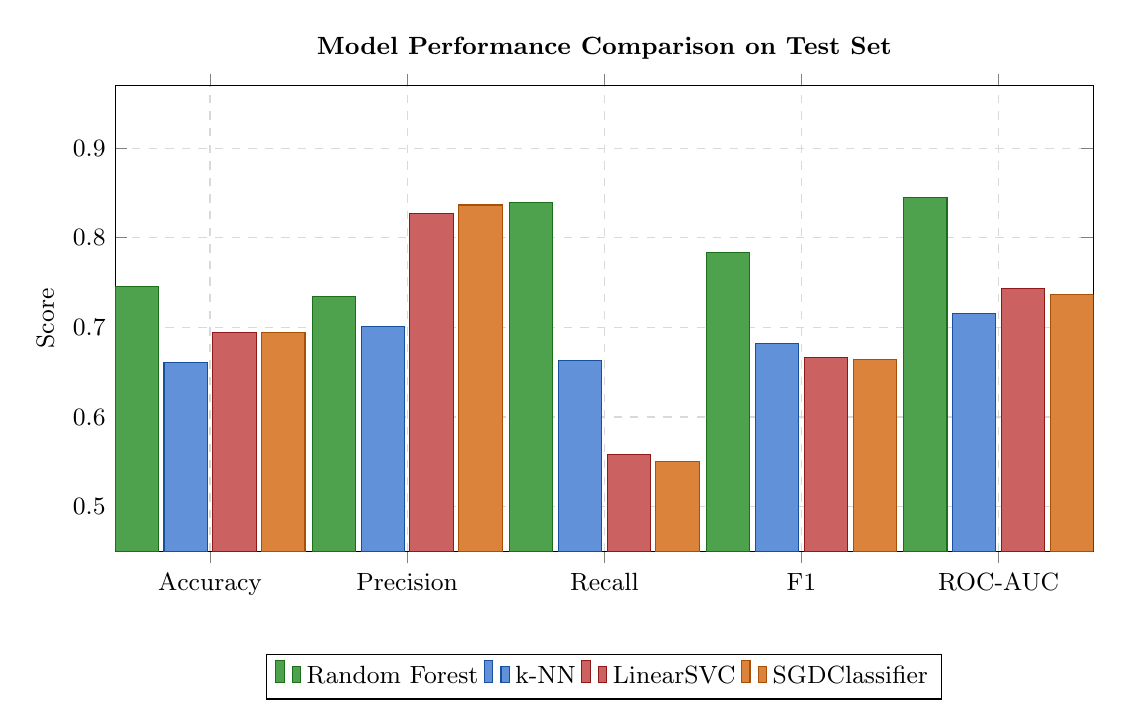
\begin{tikzpicture}
\begin{axis}[
  ybar,
  bar width=0.55cm,
  width=14cm, height=7.5cm,
  symbolic x coords={Accuracy, Precision, Recall, F1, ROC-AUC},
  xtick=data,
  ymin=0.45, ymax=0.97,
  ylabel={Score},
  ylabel style={font=\small},
  xlabel style={font=\small},
  tick label style={font=\small},
  legend style={at={(0.5,-0.22)}, anchor=north, legend columns=4, font=\small},
  enlarge x limits=0.12,
  grid=major,
  grid style={dashed,gray!30},
  title={Model Performance Comparison on Test Set},
  title style={font=\small\bfseries},
]
% Random Forest
\addplot[fill=rfgreen!80, draw=rfgreen!80!black]
  coordinates {(Accuracy,0.7455)(Precision,0.7342)(Recall,0.8397)(F1,0.7834)(ROC-AUC,0.8449)};
% k-NN
\addplot[fill=knnblue!70, draw=knnblue!80!black]
  coordinates {(Accuracy,0.6605)(Precision,0.7014)(Recall,0.6631)(F1,0.6817)(ROC-AUC,0.7158)};
% LinearSVC
\addplot[fill=svcred!70, draw=svcred!80!black]
  coordinates {(Accuracy,0.6940)(Precision,0.8274)(Recall,0.5585)(F1,0.6668)(ROC-AUC,0.7434)};
% SGD
\addplot[fill=sgdorange!80, draw=sgdorange!80!black]
  coordinates {(Accuracy,0.6944)(Precision,0.8366)(Recall,0.5500)(F1,0.6637)(ROC-AUC,0.7368)};
\legend{Random Forest, k-NN, LinearSVC, SGDClassifier}
\end{axis}
\end{tikzpicture}
\caption{Grouped bar chart comparing all five evaluation metrics across the four models on the held-out test set.}
\label{fig:grouped_bar}
\end{figure}

\subsection{F1-Score and ROC-AUC Ranking}

\begin{figure}[H]
\centering
\begin{subfigure}[b]{0.48\textwidth}
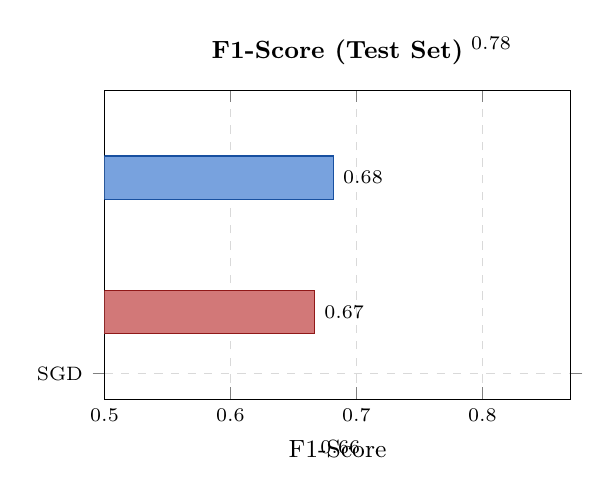
\begin{tikzpicture}
\begin{axis}[
  xbar,
  bar width=0.55cm,
  width=7.5cm, height=5.5cm,
  symbolic y coords={SGD, LinearSVC, k-NN, Random Forest},
  ytick=data,
  xmin=0.5, xmax=0.87,
  xlabel={F1-Score},
  xlabel style={font=\small},
  tick label style={font=\scriptsize},
  nodes near coords,
  nodes near coords align={horizontal},
  every node near coord/.append style={font=\scriptsize},
  grid=major,
  grid style={dashed,gray!30},
  title={F1-Score (Test Set)},
  title style={font=\small\bfseries},
]
\addplot[fill={svcred!60},  draw=svcred!80!black]
  coordinates {(0.6637,SGD)};
\addplot[fill={svcred!60},  draw=svcred!80!black]
  coordinates {(0.6668,LinearSVC)};
\addplot[fill={knnblue!60}, draw=knnblue!80!black]
  coordinates {(0.6817,k-NN)};
\addplot[fill={rfgreen!70}, draw=rfgreen!80!black]
  coordinates {(0.7834,Random Forest)};
\end{axis}
\end{tikzpicture}
\caption{F1 ranking.}
\end{subfigure}
\hfill
\begin{subfigure}[b]{0.48\textwidth}
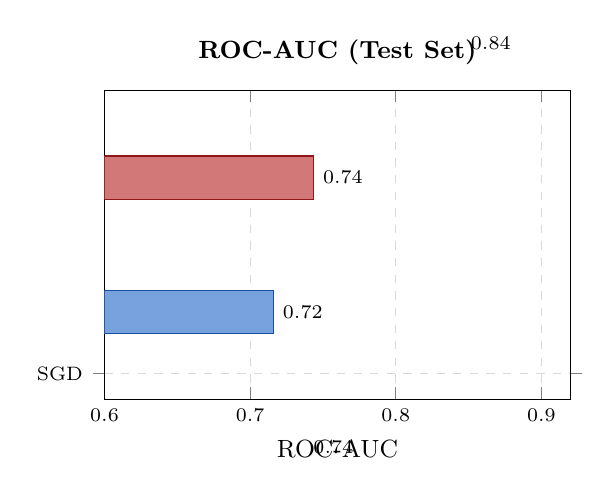
\begin{tikzpicture}
\begin{axis}[
  xbar,
  bar width=0.55cm,
  width=7.5cm, height=5.5cm,
  symbolic y coords={SGD, k-NN, LinearSVC, Random Forest},
  ytick=data,
  xmin=0.60, xmax=0.92,
  xlabel={ROC-AUC},
  xlabel style={font=\small},
  tick label style={font=\scriptsize},
  nodes near coords,
  nodes near coords align={horizontal},
  every node near coord/.append style={font=\scriptsize},
  grid=major,
  grid style={dashed,gray!30},
  title={ROC-AUC (Test Set)},
  title style={font=\small\bfseries},
]
\addplot[fill={svcred!60},  draw=svcred!80!black]
  coordinates {(0.7368,SGD)};
\addplot[fill={knnblue!60}, draw=knnblue!80!black]
  coordinates {(0.7158,k-NN)};
\addplot[fill={svcred!60},  draw=svcred!80!black]
  coordinates {(0.7434,LinearSVC)};
\addplot[fill={rfgreen!70}, draw=rfgreen!80!black]
  coordinates {(0.8449,Random Forest)};
\end{axis}
\end{tikzpicture}
\caption{ROC-AUC ranking.}
\end{subfigure}
\caption{Model rankings by primary metrics.  Random Forest leads on both.}
\label{fig:rankings}
\end{figure}

\subsection{Cross-Validation Stability}

\begin{figure}[H]
\centering
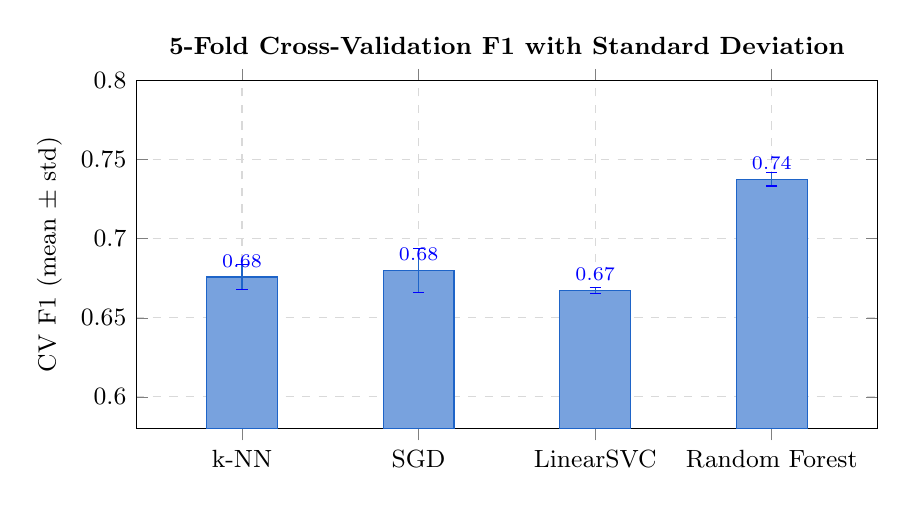
\begin{tikzpicture}
\begin{axis}[
  ybar,
  bar width=0.9cm,
  width=11cm, height=6cm,
  symbolic x coords={k-NN, SGD, LinearSVC, Random Forest},
  xtick=data,
  ymin=0.58, ymax=0.80,
  ylabel={CV F1 (mean $\pm$ std)},
  ylabel style={font=\small},
  tick label style={font=\small},
  nodes near coords,
  nodes near coords align={vertical},
  every node near coord/.append style={font=\scriptsize},
  error bars/y dir=both,
  error bars/y explicit,
  grid=major,
  grid style={dashed,gray!30},
  title={5-Fold Cross-Validation F1 with Standard Deviation},
  title style={font=\small\bfseries},
  enlarge x limits=0.2,
]
\addplot+[
  fill=knnblue!60, draw=knnblue,
  error bars/.cd, y dir=both, y explicit,
] coordinates {
  (k-NN,          0.6758) +- (0,0.0078)
  (SGD,           0.6798) +- (0,0.0139)
  (LinearSVC,     0.6672) +- (0,0.0020)
  (Random Forest, 0.7377) +- (0,0.0044)
};
\end{axis}
\end{tikzpicture}
\caption{5-fold cross-validated F1 scores with standard deviation error bars. Lower std indicates greater stability.}
\label{fig:cv}
\end{figure}

\subsection{Feature Importance (Random Forest)}

\begin{figure}[H]
\centering
\begin{tikzpicture}
\begin{axis}[
  xbar,
  bar width=0.45cm,
  width=12cm, height=8cm,
  symbolic y coords={
    Order Item Quantity,
    order\_quarter,
    Product Price,
    Shipping Mode\_Second Class,
    order\_dayofweek,
    Order Item Discount Rate,
    Order Item Discount,
    Order Item Total,
    Shipping Mode\_First Class,
    Order Item Profit Ratio,
    Order Profit Per Order,
    Longitude,
    Latitude,
    Days for shipment,
    Shipping Mode\_Std Class
  },
  ytick=data,
  xmin=0, xmax=0.085,
  xlabel={Importance score},
  xlabel style={font=\small},
  tick label style={font=\scriptsize},
  nodes near coords,
  nodes near coords align={horizontal},
  every node near coord/.append style={font=\scriptsize\color{darkgray}},
  grid=major,
  grid style={dashed,gray!30},
  title={Top 15 Random Forest Feature Importances},
  title style={font=\small\bfseries},
  enlarge y limits=0.05,
]
\addplot[fill=rfgreen!70, draw=rfgreen!80!black] coordinates {
  (0.0146, Order Item Quantity)
  (0.0174, order\_quarter)
  (0.0175, Product Price)
  (0.0178, Shipping Mode\_Second Class)
  (0.0337, order\_dayofweek)
  (0.0351, Order Item Discount Rate)
  (0.0420, Order Item Discount)
  (0.0429, Order Item Total)
  (0.0440, Shipping Mode\_First Class)
  (0.0450, Order Item Profit Ratio)
  (0.0501, Order Profit Per Order)
  (0.0547, Longitude)
  (0.0583, Latitude)
  (0.0653, Days for shipment)
  (0.0728, Shipping Mode\_Std Class)
};
\end{axis}
\end{tikzpicture}
\caption{Top 15 feature importances from the selected Random Forest model.
Shipping mode and scheduled delivery days dominate.}
\label{fig:feature_imp}
\end{figure}

\subsection{Analysis and Interpretation}

\paragraph{Random Forest vs.\ linear models.}
Random Forest achieves an F1 of 0.7834 and ROC-AUC of 0.8449, far ahead of
the three linear/linear-kernel models (best F1: 0.6817 for k-NN). The gap
confirms that delivery risk depends on \emph{non-linear interactions} between
features --- for example, the combination of shipping mode, scheduled days,
and geographic region --- which linear decision boundaries cannot capture.

\paragraph{Precision--recall trade-off.}
LinearSVC and SGD achieve notably high precision (0.83--0.84) but very low
recall (0.55--0.56). They flag few false alarms but \emph{miss} roughly 44\,\%
of truly late orders. In an operational setting this is dangerous: nearly half
of at-risk shipments would receive no intervention. Random Forest's more
balanced profile (precision 0.73, recall 0.84) is operationally preferable.

\paragraph{k-NN behaviour.}
k-NN's perfect training F1 (1.0 on the subsample, due to \texttt{weights=
'distance'} and $k=15$) versus its test F1 of 0.6817 reveals moderate
overfitting. The 25,000-sample subsample and high-dimensional feature space
(232 features) accentuate the curse of dimensionality.

\paragraph{SGD instability.}
SGD shows the highest CV standard deviation (0.0139) among all models,
indicating sensitivity to the data partition in fold-level training. This is
consistent with the online learning nature of SGD and its sensitivity to the
learning rate schedule.

\paragraph{Feature importance insights.}
The dominant features in Random Forest are:
\begin{itemize}[itemsep=2pt]
  \item \textbf{Shipping Mode} (Standard Class: 7.3\,\%, First Class: 4.4\,\%,
        Second Class: 1.8\,\%) --- carrier choice is the single strongest signal.
  \item \textbf{Days for shipment (scheduled)}: 6.5\,\% --- longer scheduled
        windows correlate with late delivery.
  \item \textbf{Geographic location} (Latitude + Longitude: 11.3\,\% combined)
        --- origin--destination geography impacts carrier reliability.
  \item \textbf{Financial metrics} (profit, discounts): moderate but
        consistent contribution, suggesting order prioritisation effects.
\end{itemize}

\subsection{Final Model Selection}

\begin{table}[H]
\centering
\caption{Decision scorecard for final model selection.}
\label{tab:selection}
\renewcommand{\arraystretch}{1.25}
\begin{tabular}{lcccc}
\toprule
\textbf{Criterion} & \textbf{RF} & \textbf{k-NN} & \textbf{LinearSVC} & \textbf{SGD} \\
\midrule
Highest F1 (test)       & \checkmark &  &  &  \\
Highest ROC-AUC         & \checkmark &  &  &  \\
Highest Recall          & \checkmark &  &  &  \\
Lowest CV std           & \checkmark &  &  &  \\
Balanced precision/recall & \checkmark & partial &  &  \\
Non-linear capacity     & \checkmark &  &  &  \\
Interpretable (feature importance) & \checkmark &  &  &  \\
\midrule
\textbf{Score} & \textbf{7/7} & 1/7 & 0/7 & 0/7 \\
\bottomrule
\end{tabular}
\end{table}

\textbf{Selected model: Random Forest} with
\texttt{n\_estimators=100}, \texttt{max\_depth=None},
\texttt{min\_samples\_leaf=1}, \texttt{max\_features='sqrt'}.

\subsection{Inference on Unseen Orders}

The Random Forest was applied to the 10 orders held out before preprocessing
to simulate production inference. Table~\ref{tab:inference} reports the true
label, predicted label, and estimated late-delivery probability.

\begin{table}[H]
\centering
\caption{Inference results on 10 unseen production orders.}
\label{tab:inference}
\renewcommand{\arraystretch}{1.25}
\begin{tabular}{ccccl}
\toprule
\textbf{Order \#} & \textbf{True Label} & \textbf{Predicted} & \textbf{$P(\text{Late})$} & \textbf{Correct?} \\
\midrule
0  & Late (1)     & On-Time (0) & 0.50 & \textcolor{svcred}{No}  \\
1  & Late (1)     & Late (1)    & 0.99 & \textcolor{rfgreen}{Yes} \\
2  & On-Time (0)  & On-Time (0) & 0.26 & \textcolor{rfgreen}{Yes} \\
3  & Late (1)     & On-Time (0) & 0.41 & \textcolor{svcred}{No}  \\
4  & On-Time (0)  & On-Time (0) & 0.43 & \textcolor{rfgreen}{Yes} \\
5  & Late (1)     & On-Time (0) & 0.37 & \textcolor{svcred}{No}  \\
6  & Late (1)     & Late (1)    & 0.58 & \textcolor{rfgreen}{Yes} \\
7  & On-Time (0)  & On-Time (0) & 0.37 & \textcolor{rfgreen}{Yes} \\
8  & Late (1)     & On-Time (0) & 0.50 & \textcolor{svcred}{No}  \\
9  & On-Time (0)  & On-Time (0) & 0.40 & \textcolor{rfgreen}{Yes} \\
\midrule
\multicolumn{2}{l}{\textbf{Accuracy}} & \multicolumn{3}{l}{6/10 = 60\,\%} \\
\multicolumn{2}{l}{\textbf{Mean $P(\text{Late})$}} & \multicolumn{3}{l}{0.481} \\
\bottomrule
\end{tabular}
\end{table}

The 6/10 inference accuracy is lower than the test-set accuracy of 74.6\,\%.
This is expected: 10 samples is a very small evaluation set, and all four
misclassifications involve ambiguous orders with $P(\text{Late}) \in [0.37,
0.50]$ --- i.e., near the decision boundary. In a production system, orders
with predicted probability above a tunable threshold (e.g., $P > 0.40$) could
be flagged for human review, converting borderline predictions into risk alerts
rather than hard binary decisions.

Figure~\ref{fig:inference_probs} visualises the predicted probabilities
alongside the true labels.

\begin{figure}[H]
\centering
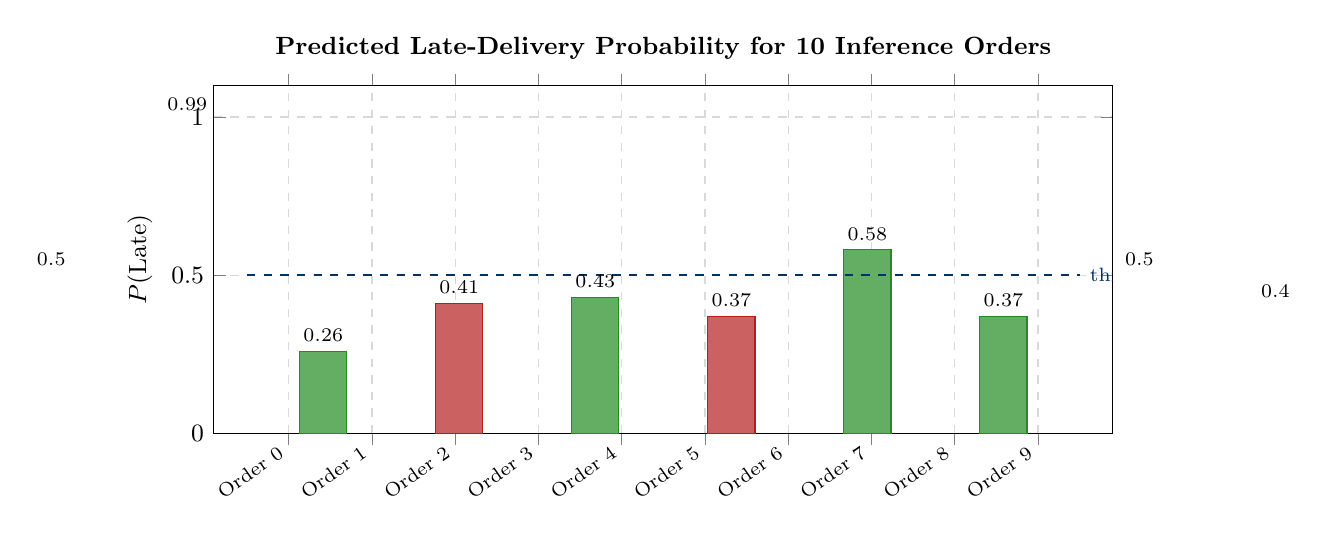
\begin{tikzpicture}
\begin{axis}[
  ybar,
  bar width=0.6cm,
  width=13cm, height=6cm,
  xtick={0,1,2,3,4,5,6,7,8,9},
  xticklabels={Order 0, Order 1, Order 2, Order 3, Order 4,
               Order 5, Order 6, Order 7, Order 8, Order 9},
  x tick label style={rotate=35,anchor=east,font=\scriptsize},
  ymin=0, ymax=1.1,
  ylabel={$P(\text{Late})$},
  ylabel style={font=\small},
  tick label style={font=\small},
  nodes near coords,
  nodes near coords align={vertical},
  every node near coord/.append style={font=\scriptsize},
  grid=major,
  grid style={dashed,gray!30},
  title={Predicted Late-Delivery Probability for 10 Inference Orders},
  title style={font=\small\bfseries},
]
% Colour: green = correct, red = incorrect
\addplot[fill=svcred!70,  draw=svcred]  coordinates {(0,0.50)};  % wrong
\addplot[fill=rfgreen!70, draw=rfgreen] coordinates {(1,0.99)};  % correct
\addplot[fill=rfgreen!70, draw=rfgreen] coordinates {(2,0.26)};  % correct
\addplot[fill=svcred!70,  draw=svcred]  coordinates {(3,0.41)};  % wrong
\addplot[fill=rfgreen!70, draw=rfgreen] coordinates {(4,0.43)};  % correct
\addplot[fill=svcred!70,  draw=svcred]  coordinates {(5,0.37)};  % wrong
\addplot[fill=rfgreen!70, draw=rfgreen] coordinates {(6,0.58)};  % correct
\addplot[fill=rfgreen!70, draw=rfgreen] coordinates {(7,0.37)};  % correct
\addplot[fill=svcred!70,  draw=svcred]  coordinates {(8,0.50)};  % wrong
\addplot[fill=rfgreen!70, draw=rfgreen] coordinates {(9,0.40)};  % correct
% Decision threshold
\draw[dashed,thick,mitblue] (axis cs:-0.5,0.5) -- (axis cs:9.5,0.5)
  node[right,font=\scriptsize,color=mitblue] {threshold};
\end{axis}
\end{tikzpicture}
\caption{Predicted late-delivery probabilities for 10 held-out inference orders.
Green = correct prediction; red = incorrect. Dashed line marks the 0.5 decision threshold.}
\label{fig:inference_probs}
\end{figure}

% ══════════════════════════════════════════════════════════════════════════════
\section{Conclusion}
\label{sec:conclusion}

This project developed and compared four machine learning models for binary
classification of late delivery risk in supply chain logistics, using
180,509 real-world orders from the DataCo Global dataset.

The key findings are:

\begin{itemize}[itemsep=3pt]
  \item \textbf{Random Forest is the best model} across all five evaluation
        metrics (F1: 0.78, ROC-AUC: 0.84), with the most stable
        cross-validation performance (CV std: 0.004).
  \item \textbf{Linear models (LinearSVC, SGD) over-predict precision at the
        cost of recall}, flagging too few at-risk orders for operational use.
  \item \textbf{Shipping mode and scheduled delivery time} are the strongest
        predictors, followed by geographic coordinates and profit metrics.
  \item \textbf{Near-boundary predictions} ($P \approx 0.4$--$0.5$) represent
        genuinely uncertain orders; a softened threshold strategy can convert
        these into actionable risk alerts.
\end{itemize}

Future improvements could include gradient boosted trees (XGBoost / LightGBM),
SMOTE-based oversampling for the minority class, and threshold calibration
optimised for the specific cost ratio of false negatives to false positives in
the operational context.

% ══════════════════════════════════════════════════════════════════════════════
\section*{References}
\addcontentsline{toc}{section}{References}

\begin{enumerate}[label={[\arabic*]},leftmargin=2.5em,itemsep=4pt]
  \item Constante, F., Silva, F., \& Pereira, A. (2019).
        \textit{DataCo Smart Supply Chain for Big Data Analysis} [Dataset].
        Mendeley Data. \url{https://doi.org/10.17632/8gx2fvg2k6.5}
  \item Breiman, L. (2001). Random Forests.
        \textit{Machine Learning}, 45(1), 5--32.
  \item Cortes, C., \& Vapnik, V. (1995). Support-vector networks.
        \textit{Machine Learning}, 20(3), 273--297.
  \item Cover, T., \& Hart, P. (1967). Nearest neighbor pattern classification.
        \textit{IEEE Transactions on Information Theory}, 13(1), 21--27.
  \item Bottou, L. (2010). Large-scale machine learning with stochastic
        gradient descent. \textit{COMPSTAT}, 177--186.
  \item Pedregosa, F., et al. (2011). Scikit-learn: Machine learning in Python.
        \textit{JMLR}, 12, 2825--2830.
\end{enumerate}

\end{document}
